\documentclass[tikz,border=10pt]{standalone}
\begin{document}
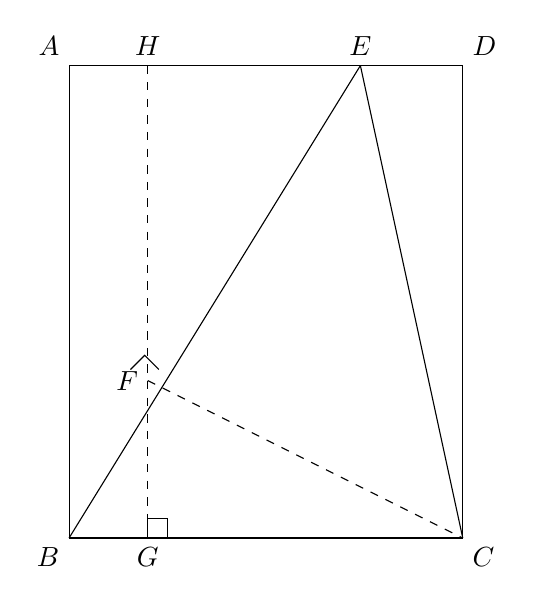
\begin{tikzpicture}[scale=1]

\coordinate (A) at (0,6);
\coordinate (B) at (0,0);
\coordinate (C) at (5,0);
\coordinate (D) at (5,6);
\coordinate (E) at (3.7,6);
\coordinate (H) at (1,6);
\coordinate (G) at (1,0);
\coordinate (F) at (1,2);

\draw (A) -- (B) -- (C) -- (D) -- cycle;
\draw (A) -- (D);
\draw (B) -- (E);
\draw (E) -- (C);

\draw[dashed] (H) -- (G);
\draw[dashed] (F) -- (C);

\draw (G) -- ++(0,0.25) -- ++(0.25,0) -- ++(0,-0.25);
\draw (F) ++(0.14,0.14) -- ++(-0.18,0.18) -- ++(-0.18,-0.18);

\node[above left] at (A) {$A$};
\node[below left] at (B) {$B$};
\node[below right] at (C) {$C$};
\node[above right] at (D) {$D$};
\node[above] at (E) {$E$};
\node[left] at (F) {$F$};
\node[below] at (G) {$G$};
\node[above] at (H) {$H$};

\end{tikzpicture}
\end{document}
